
\chapter{Fundamental Concepts}
\label{cha:fundamentals}
\textbf{TODO: I -> We, no need to always say will, sometimes use passive to switch it up}
In this chapter we lay out the fundamental concepts, which are necessary in order to understand the subsequent chapters.
First we explain Stream Processing in \ref{sec:stream-processing}, afterwards the concept of the self-adaptive systems will be presented and explained in section \ref{sec:self-adaptive} 
followed by a brief explanation of the MAPE-K loop in \ref{sub:mape} to conclude this chapter.

    \section{Stream Processing}
    \label{sec:stream-processing}
    In this section we will split the concept of stream processing into three further components.
    In \ref{sub:sps} we will then define stream processing systems, explain how they work and give examplary fields of application.
    Afterwards in \ref{sub:dsms} we will move onto the topic of data stream management systems and finally in \ref{sub:requirements} we talk about
    some requirements that SPSs should meet.
    
        \subsection{Data Stream Management Systems}
        \label{sub:dsms}
        \ifbool{final}{}{\textbf{\color{green}THIS IS FINAL}
        
        }
        % - Streams not saved to disk (Saving to disk and retrieving has high latency), instead kept in memory (low latency)
        % - Some data might still be archived, however it does not impact performance, as it is done parallel to the streaming processing
        % - Sometimes access to archived data in DBMS needed, however this can be cached or efficiently accessed

        \begin{figure}[h]
            \label{fig:dbms_dsms}
            \centering
            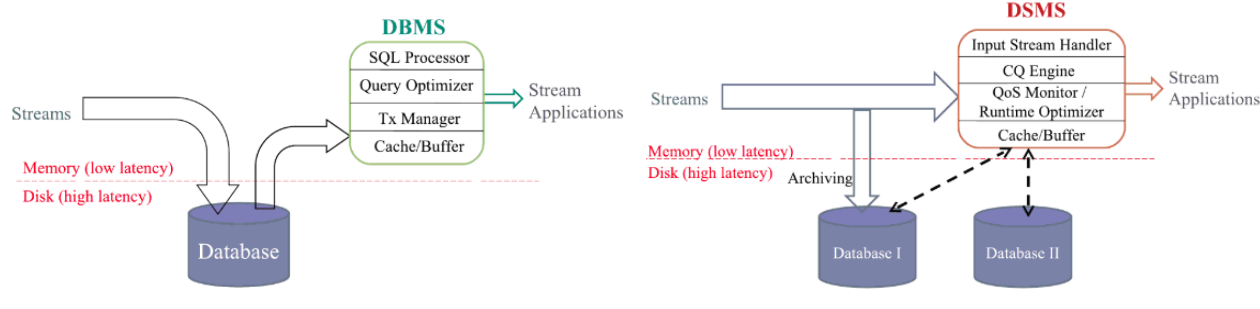
\includegraphics[width=1.0\textwidth]{Bilder/dbms_dsms.png}
            \caption{
                   left: architecture of a DBMS; right: architecture of a DSMS
                   }
        \end{figure}

        A data stream management system is a tool designed to manage continuous data streams.
        DSMSs are comparable to DBMS, however, there are differences one must take note of.

        \quad Most notably the data being fed into a DSMS varies greatly from the data being inserted into a DBMS; while a DBMS receives a finite predetermined amount 
        of data, a DSMS can theoretically receive an infinite continuous stream.
        \\
        Secondly, DSMSs operate at a much greater speed than traditional DBMSs, because the data is processed immediately, while in the DBMS approach
        data is first saved to a disk and then queried before further processing can occur, leading to two I/O actions. This behavior, coupled with an incoming 
        high velocity stream, might lead to lags or even failure to yield accurate results\cite{StreamBookQuality}. 
        However, a DSMS might want to archive certain elements from the stream. For this, there are two possibilities;
        Either data is being cached in memory, yielding much faster query results, or it is archived in additional databases parallel to the streaming process.
        Thus the DSMS architecture is superior to the DBMS architecture when measuring latency.
        When data is stored, often only synopses are stored, in an attempt to summarize the data and utilize that knowledge in form of a \gls{state} for the queries.
        The difference in these architectures is also shown in figure \ref{fig:dbms_dsms}\cite{StreamBookQuality}.
        \\
        Thirdly, similar to a DBMS a DSMS can also be queried using a streaming query language, however, queries installed on a DSMS are continuous 
        and will be executed as long as it is uninstalled and there are restrictions on which operations can be executed.
        Since the system can not assume a finite amount of data, it processes each data item as it arrives, so operators that require the entirety of a data 
        set, such as the \textit{join, aggregation} operators, prove problematic when it comes to streams, 
        as they can only return a result once the stream has ended\cite[p.12]{StreamBookQuality}.
        These queries are refered to as \textit{blocking} queries. In order to use them, one must convert them into non-blocking queries.
        One solution for this has been introduced in the form of windows, which are explained in \ref{sub:sps} \nameref{sub:sps}.

        \quad There are a few more functional differences, which Panigati, Schreiber and Zaniolo highlight, as shown in table 2.1.

        \begin{table}[h]
            \centering
            \label{tab:dbms-dsms}
            \begin{tabular}{|c|c|c|} \hline
                \textbf{Feature} & \textbf{DBMS} & \textbf{DSMS} \\ \hline
                Model & Persistent data & Transient Data \\ \hline
                Table & Set or bag of tuples & Infinite sequence of tuples \\ \hline
                Updates & All & Append only \\ \hline
                Queries & Transient & Persistent \\ \hline
                Query answers & Exact & Often approximate \\ \hline
                Query evaluation & Blocking and non-blocking & Non-blocking \\ \hline
                Operators & Fixed & Adaptive \\ \hline
                Data processing & Synchronous & Asynchronous \\ \hline
                Concurrency overhead  & High & Low \\ \hline
            \end{tabular}
            \captionbelow{Functional comparison of DBMS and DSMS\cite{Panigati2015}} 
        \end{table}

        \subsection{Stream Processing Systems}
        \label{sub:sps}
        \ifbool{final}{}{\textbf{\color{red}THIS IS NOT FINAL}
        
        }
        \textbf{TODO: Explain big data -> batch(latency low prio) and stream(latency high prio) }
        % Erklärung von Windows irgendwie einbringen (Hier noch überlegen wo am besten)
        % Erklären wozu SPS eingesetzt
        % Challenges, die SPSs facen

        % Topical sentence
        In this section we will define stream processing systems, expound what data looks like in SPS. We also explain what SPSs
        are capable of and give an example of a SPS. Furthermore windows will be explained and the concept of adaptation in SPSs will be laid out.
        In the end of the section we will present some of the challenges that SPSs face.

        % Todo: Batch processing kurz erläutern, higher latency b/c larger amounts of data are processed at once??
        \quad Stream processing systems are systems designed to handle large amounts of data in (near) real-time fashion with low latency. 
        The data is fed to the system in form of streams, which are defined as an potentially infinite, countable amount of \textit{data tuples}. 
        The streams usually originate from a \texit{data source} which, for example, can be a type of sensor, e.g. a simple temperature sensor or more complex sensors, 
        such as an EEG-sensor, market orders or network traffic.
        \\
        A data tuple is an object whose internal structure is defined by a \texit{data scheme}. 
        Objects of a data stream share a common structure, also called \textit{stream schema}.
        Tuples consist of a set of typed attributes and their respective values. One can imagine a tuple as a java object without any operations.\cite{fundamentals}
        Each individual data tuple is processed by one or more \textit{operators}.
        An operator is fed tuples from incoming streams through its input port, performs an operation and generates an output stream through its output port, 
        consisting of the processed tuples. Operators are able to perform various different operations, 
        as shown in \cite[p.49]{fundamentals}, some of which include: aggregation, splitting and merging streams, 
        logical and mathematical operations and custom data manipulations.
        \\
        The results of a streaming application is then fed into one or multiple \textit{data sinks}, which could for example be a data visualization engine 
        or an automated stock trading engine.
        
        \quad In order for a SPS to perform as fast as possible, it should have the ability to adapt to situations.
        There are many strategies of adaptation, which can be broken down into three subcategories; \textit{processing-}, \textit{data-} and 
        \textit{resource adaptation} \cite[p.8 f.]{QIN20191}. 
        An examplary resource adaptation would be a \textit{processing scaling} adaptation, as shown in figure \ref{fig:sps_parallel_normal}, 
        where, if computational resources allow it, an operator may be replicated in order to process data faster by
        making use of the principle of parallelity. Technically, there should be a splitting operator placed before, 
        as well as a merging operator after the replicated note. These have been left out for the sake of brevity.
        \\
        An example for data adaptation would be \textit{load shedding}, a strategy where some data tuples are dropped in order to free up computational resources.
        However, one must take into consideration that one possibly sacrifices accuracy for the sake of performance, as more data generally leads to more accurate results.
        Furthermore, one must take note of the resource cost to calculate which tuples to drop in order to have the lowest impact on the quality of service.
        % TODO Maybe an example here for load shedding?
        \\
        For resource adaptation we will look at \textit{dynamic resource allocation}. Dynamic resource allocation is a stratey, in which the available computational 
        resources are constantly reassigned, so as to allocate the memory in the most efficient way. For example a node facing a high data load at the moment might 
        be allocated more RAM, GPU or CPU power in order to process its load faster. For this to work some resources have to be freed first, e.g. by deducting some
        computational power from a node facing less input at the time. With this strategy, one must take into consideration the resources and time spent calculating 
        the optimal allocation of resources.



        \begin{figure}[h]
            \label{fig:sps_parallel_normal}
            \centering
            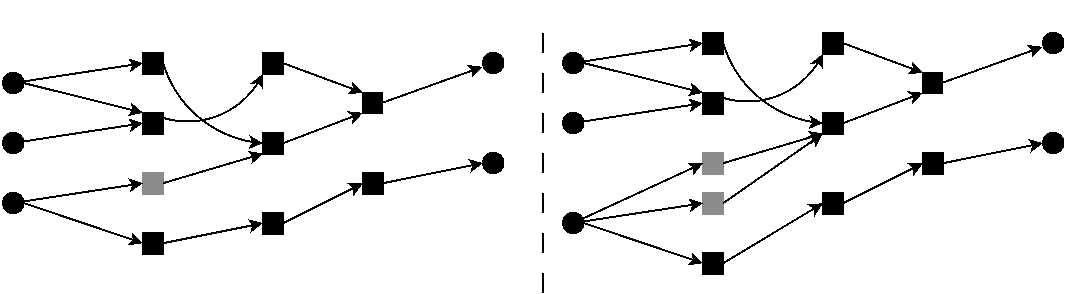
\includegraphics[width=1.0\textwidth]{Bilder/sps_parallel_normal.png}
            \caption{
                    Left: An example for an SPS displayed as a directed acyclic graph;
                    Right: Same SPS with introduced parallelity in one operator, marked gray for visibility;
                    Circles on the left depict data sources, circled on the right depict data sinks, squares are operators/processors, and arrows are streams.
                    }
        \end{figure}

        \begin{figure}

        \label{fig:stream-processing-system}
        \centering
        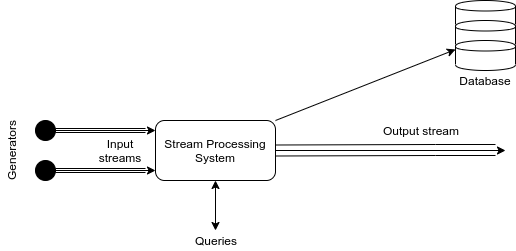
\includegraphics[width=1.0\textwidth]{Bilder/stream-processing-system.png}
        \caption{
                Overview of a basic Stream Processing System
                }
        \end{figure}  

        % Subsection Requirements for Stream Processing Systems
        % Should quickly go over the requirements and explain why they matter to us
        \subsection{Requirements for Stream Processing Systems}
        \label{sub:requirements}
        \ifbool{final}{}{\textbf{\color{red}THIS IS NOT FINAL}
        
        }

        Notes: What are the requirements, why do they matter to us (Elaborate on this)

        Due to the nature of the fields in which SPS are used, there are important requirements that SPS should meet in order to be viable, 
        which Stonebraker et al. point out in \cite{Stonebraker:2005:RRS:1107499.1107504}, of which the ones most important to us can be summarized as the following:
        
        % Enumeration of requirements for SPS + explanations why they matter to us
        \begin{enumerate}
        \label{enum:requirements}
            \item \textbf{Keep the Data Moving:} 
                In order to minimize latency, data must not be stored, as these are costly operations.
            \item \textbf{Handle Stream Imperfections:} 
                Expecting only perfect data is utopian, so one must prepare the system with built-in mechanisms for data that might be missing or out-of-order.
            \item \textbf{Integrate Stored and Streaming Data:} 
                For an SPS to be able to perform comparisons between "predecessor" data and current data, operators must keep an efficiently manageable state.
            \item \textbf{Guarantee Data Safety and Availability:} 
                Recovering from a failure is detrimental for real-time data processing, so a system must be in place to guarantee the highest availability possible.
            \item \textbf{Process and Respond Instantaneously:} 
                Systems must be highly optimized in order to provide (near) real-time responses.
            \item \textbf{Partition and Scale Applications Automatically:} 
                Systems must be able to be split across multiple machines and threads.
                The system must also be able to automatically scale and distribute the load across the machines.

        \end{enumerate}

    \section{Self-Adaptive Systems}
    \label{sec:self-adaptive}
    \ifbool{final}{}{\textbf{\color{green}THIS IS FINAL?}
    
    }{}
    
    % \textbf{TODO: Needs more; e.g why self-adaptive(already mentioned in intro), Software engineering perspective on self adaptivity, challenges}
    % Definition of self-adaptive systems
    % Architecture often based on mape in different patterns
    % applied in xx industries
    Cheng et al. define self-adaptive systems as
    \begin{quotation}
        ``[...] systems that are able to adjust their behaviour in response to their perception of the environment and the
        system itself [...]``\cite[p.1]{Cheng:2009:SES:1573856.1573858}.
    \end{quotation}
    
    Self-adaptive systems are oftentimes based on the \nameref{sub:mape} [p.\pageref{sub:mape}] pattern.
    Adaptive Systems have a wide variety of possible application areas: adaptable user interfaces, autonomic computing, multi-agent systems \cite{Cheng:2009:SES:1573856.1573858}, 
    biologically inspired computing, robotics \cite{10.1007/978-3-319-59480-4_44}, streaming applications and a lot more.

    An examplary application would be a scenario, in which population and food capacities are given and evolving over time, due to births, deaths, changes in demographics 
    and changes in weather and harvest respectively. A system would have to adapt to these changes in its environment in order to ration the food properly.

    
    \subsection{MAPE-K Loop}
    \label{sub:mape}
    \ifbool{final}{}{\textbf{\color{green}THIS IS FINAL (Maybe add something underneath enum if not sufficient)}
    
    }{}
    % Explain the MAPE-K Loop as it is a valuable basis/reference architecture for many different approaches in adaptive systems
    % Rough explanation of what it is, where it is used
    % explain different "stages" (m, a, p, e)
    % Explain -K extension
    The MAPE-K Loop was introduced by IBM \cite{Kephart:2003:VAC:642194.642200} and refers to a proposed solution for self-adaptive or autonomic systems.
    This model has since become the basis or reference architectural pattern for many self adaptive systems, which I will show in the third chapter.
    The acronym MAPE-K refers to the components that make up the model:
    \textbf{TODO: Add a diagram, make this a subsection of self-adaptive systems}
     \begin{figure}[hbt]
        \label{fig:mape}
        \centering
        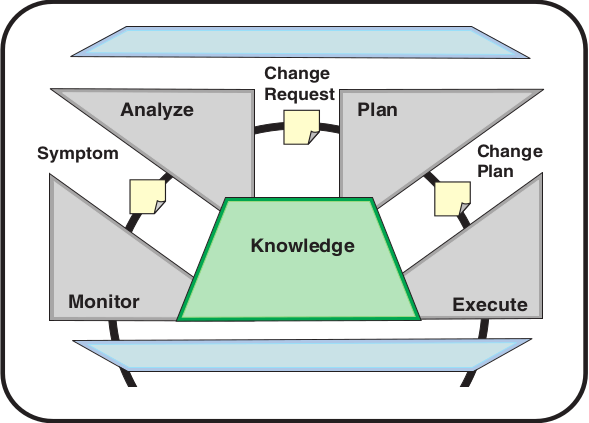
\includegraphics[width=0.45\textwidth]{Bilder/mape.png}
        \caption{
                Overview of the MAPE-K-Loop\cite{Kephart:2003:VAC:642194.642200}
                }
    \end{figure}  
    \begin{enumerate}
    \label{enum:mape}
        \item \textbf{M}onitor: 
            The \textit{Monitor} component gathers data about the system and its environment, aggregates and filters it.
        \item \textbf{A}nalyze: 
            The \textit{Analyze} component analyzes the previously gathered data and determines whether or not an adaptation should be performed.
            The decision is made based on performance or cost gain and should include the adaptation cost as well.
            This component's analysis is influenced by the \textit{Knowledge} base.
        \item \textbf{P}lan: 
            If the choice to adapt the system has been made, the \textit{Plan} component then decides how to reconfigure the system.
            Once the decision has been made, the information is then forwarded to the \textit{Execute} component.
        \item \textbf{E}xecute: 
            Given the \textit{Plan} component's decision, the \textit{Execute} component then executes said plan and the loop 
            returns to the initial monitoring state.
        \item \textbf{K}nowledge: 
            Represents the knowledge base, which is shared between the other components.
            This base is created by the \textit{Monitor} component and contains information in the form of metrics, policies, symptoms and logs.
    \end{enumerate}
   


\chapter{Approaches for Self-Adaptive Architectures in Stream Processing}
\label{cha:approaches}
\textbf{TODO: How does it work? FOCUS ON ARCHITECTURE IN THIS CHAPTER!!}
Explain that this chapter showcases a few select strategies, which are then elaborated on further in the subchapters
Question: Even more approaches? e.g. Master-Slave pattern or Coordinated Control pattern (Both MAPE based)?
\textbf{Add and explain a few more MAPE Based architectures}

    \section{Dhalion}
    \label{sec:dhalion}
    Quick Introduction to Dhalion, this chapter will deal with the Dhalion paper.
    NOTE: Explain what Dhalion is, where its used

        \subsection{An Outline of Heron}
        \label{sub:heron-outline}
        Small outline of Heron, as Dhalion is built on top of Twitter's Heron.

        \subsection{Dhalion's Architecture}
        \label{sec:dhalion-architecture}
        \textbf{TODO: Diagram, explain it here}
        Explanation of Dhalion's Architecture \textbf{KERNPUNKT DER SECTION DHALION}

        \subsection{Discussion of Dhalion}
        \label{sec:dhalion-discussion}
        Discuss the approach and compare it to the reference architecture (Mape?)
        \textbf{TODO: Maybe discuss how they evaluate, look at metrics relevant to architecture}

    \section{Decentralized Self-Adaptation}
    \label{sec:hierarchical}
    \textbf{TODO: Incorporate same structure as above}
    NOTE: In this section I will explain the hierarchical control architecture as decribed by Cardellini..

        \subsection{Elastic and Distributed DSP Framework}
        \label{sec:edf}
        \textbf{TODO: Possibly change title of this, add diagram, explain thoroughly (decentralized etc.), extract their design patterns}
        Explanation of the EDF, their architecture for elastic DSP apps \textbf{KERNPUNKT DER SECTION}

        \subsection{Discussion of EDF}
        \label{sec:discussion-edf}

    \section{Some Other Architecture}
    \label{sec:soa}
    NOTE: In this chapter I will explain another architecture/approach to self-adaption, yet to be researched


    \section{Some Other Architecture2}
    \label{sec:soa2}
    NOTE: In this chapter I will explain another architecture/approach to self-adaption, yet to be researched


    \section{Title??}
    \textbf{TODO: Discuss among all of them, critical thinking..}

    \textbf{TODO: If enough material compare the architecture relevant metrics of the approaches}